\section{A headless pipeline on a laptop}
\label{sec:pipeline}

\subsection{Setup}
Everything in this section ran on a MacBook Air (Apple Silicon, 16\,GB) on 14 October 2026, streaming data from \code{s3://vesuvius-challenge-open-data}. The target is PHerc1447, volume \code{20250521151220} at \SI{8.64}{\um}, with the organisers' April 2026 surface prediction (\code{surface-m7-L0-}\allowbreak\code{th0.2}) as the seed field. The command-line tools \code{vc\_grow\_seg\_from\_seed} and \code{vc\_render\_tifxyz} are taken from the VC3D application bundle (build \code{afdb836}, 14 October 2026); ink inference uses the \code{vesuvius} package from the ScrollPrize \code{villa} repository (commit \code{5432721}) in a slim virtual environment with PyTorch on the Metal (MPS) backend and no compiled extensions. Every run is driven by a shell script that logs the command, the build and the wall time.

\subsection{Seeds}
Seeds are drawn from the level-3 pyramid of the surface prediction (\SI{1}{/8} resolution, about \SI{2}{MB} read), uniformly at random with a minimum separation of 600 voxels. Two things went wrong before anything grew.

\begin{enumerate}
\item Seeding from the vertices of the team's May 2025 patches put the tracer off the April 2026 prediction (the prediction value at those vertices was zero). The tracer then started in the gap and produced swirling, sheet-crossing patches. Seeds must come from the \emph{current} prediction.
\item The first prediction-only seed grew \SI{1.35}{cm^2} in \SI{534}{s} and rendered to all zeros: it lay outside the masked scroll. Counting at level 3, the prediction has $39.5\times10^6$ surface voxels, of which only $13.2\times10^6$ (34\,\%) sit where the masked CT exceeds 20. Two thirds of the surface field is outside the object it is meant to describe. A CT mask was added to the seed picker.
\end{enumerate}

\subsection{Grow, render, inspect}
\Cref{tab:seeds} lists the seeds grown with the tracer at 35 generations and rendered as 28 layers at step 1 (the window the \SI{9}{\um} ink model expects). \code{composite.py} writes a maximum-intensity projection, the middle layer and a contact sheet; \code{qa.py} samples a $3\times3$ grid of mesh points and draws the CT cross-sections through each with the mesh overlaid (\cref{fig:contact}). The cross-sections caught a failure the flattened images did not: for seed 5452 the top third of a visually clean patch lies in air, where the tracer overgrew the outer wrap.

\begin{table}[t]
\centering\small
\caption{Patches grown on PHerc1447. Grow time is for \code{vc\_grow\_seg\_from\_seed} alone. Verdicts are from the contact sheet and the cross-section QA.}
\label{tab:seeds}
\begin{tabular}{@{}lrl@{}}
\toprule
seed $(x,y,z)$ & grow [s] & verdict \\
\midrule
5452 4100 22772 & 107 & clean weave; top third in air \\
3532 4492 23020 & 375 & clean; sheet switch, lower left \\
2388 3356 22308 & 212 & mixed \\
3092 6212 22708 & 76  & mixed \\
7036 4612 24060 & 167 & reject: compressed mass \\
4020 1948 24284 & 63  & reject: edge, 11\,\% fill \\
4144 2742 12557 & 145 & announced text site; 9/9 QA points on sheet \\
\bottomrule
\end{tabular}
\end{table}

\begin{figure}[t]
\centering
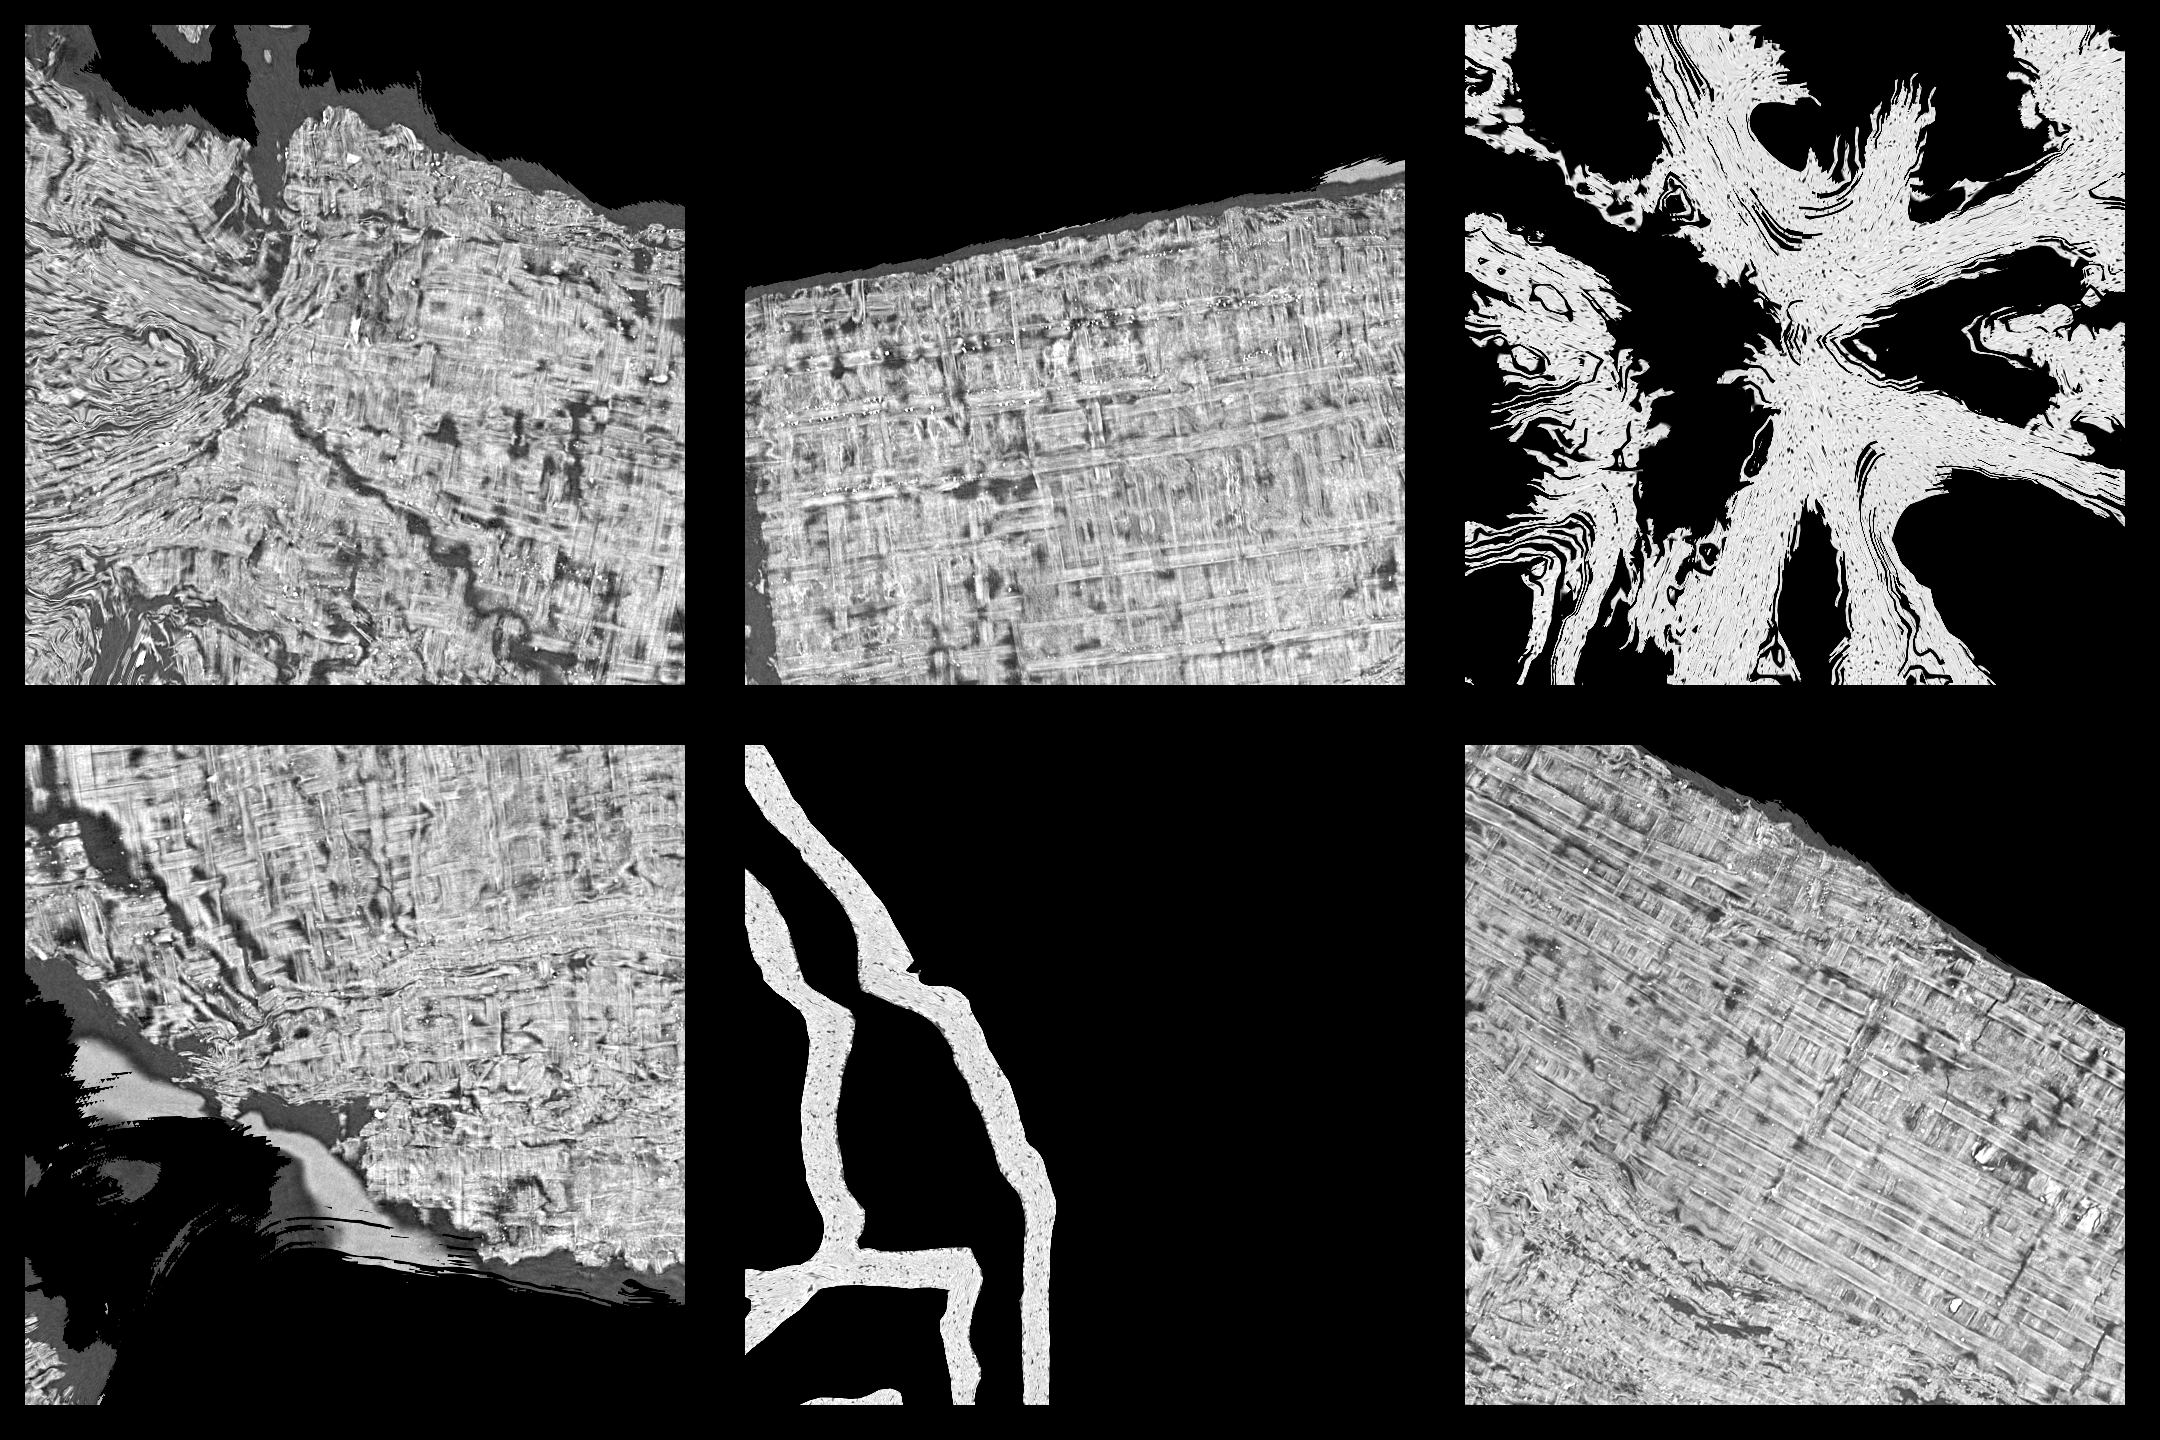
\includegraphics[width=\linewidth]{_contact_run3}
\caption{Contact sheet for the six in-scroll seeds of the third run (middle layer of each render). Two are clean, two mixed, two rejected. The lower-left region of 3532 is the sheet switch analysed in \cref{sec:holonomy,sec:tetratic}.}
\label{fig:contact}
\end{figure}

\paragraph{Failure modes found.} Stale seeds off the current prediction; prediction voxels outside the scroll mask; overgrowth into air past the outer wrap; and the sheet switch that motivates the rest of this note.
